\chapter{\label{ch:5-CHECNSB} Advanced Study of SSTCAM NSB}
\minitoc
\begin{abstract}
    Night Sky Background (NSB) is a complex phenomenon, consisting of all light detected by imaging atmospheric Cherenkov telescopes not attributable to Cherenkov light emission. Understanding the effect of NSB on cameras for the next-generation Cherenkov Telescope Array (CTA) is important, as it affects the astrophysical systematic errors on observations, the ability of the telescopes to operate under partial moonlight conditions and the thermal control of the cameras. The capacity to observe under partial moonlight conditions is crucial for the CTA transient science programme, as it substantially increases the potential observing time. Using tools initially developed for H.E.S.S. (in combination with the prototype CTA analysis package ctapipe) we will present predictions for the NSB present in images taken by the Small Sized Telescope Camera (SSTCAM), showing that SSTCAM will likely be able to meet the associated CTA requirements. Additionally, we calculate the potential observing time gain by operating under high NSB conditions.
\end{abstract}

\section{Introduction}
\label{sec:intro}

\subsection{Scope \& Purpose of this Chapter}
\label{sec:intro:scope}
As we've seen in Chapters \ref{ch:3-TimingInfo} and \ref{ch:4-VERITASRealData}, it is possible that the current modelling of NSB in both the simulation packages \textit{CARE} (used by VERITAS and in Chapter \ref{ch:4-VERITASRealData}) and \textit{sim\_telarray} (used by CTA and H.E.S.S. and in Chapter \ref{ch:3-TimingInfo}) is insufficient to allow for reliable deep-learning-based event classification. In this chapter, we estimate the expected NSB photon rates of SSTCAM under various observing conditions. This modelling will aid SSTCAM design, as well as begin a possible route to improvement in our training data that might one day make deep learning analyses feasible. We perform this by using and expanding upon the capabilities of the \textit{nsb} tool \cite{nsb}, already validated and used by H.E.S.S.. For the purposes of this chapter, capitalised NSB refers to the physical phenomenon of Night Sky Background, where as italic lower case \textit{nsb} refers to the Python package used to simulate it. Full results from this study, along with sandbox scripts to operate \textit{nsb} can be found on the \url{https://github.com/sstcam/sstcam_NSB} Github page. 

\subsection{Context}
\label{sec:intro:context}
The ability for SSTCAM to operate reliably under partial moonlight and other high NSB observing conditions is critical to the transient and multi-messenger/multi-wavelength science goals of CTA. This is as operating under these conditions significantly increases the possible observing time, and so this ability has been designated as a CTA system requirement.  The increase in potential science return was judged to outweigh the associated increase in data rate and person-power required. The most notable justification for this is the detection of prompt TeV emission from GRB 190114C (the first such detection from the ground) under partial moonlight conditions (6 times nominal NSB) with MAGIC \cite{magicGRB}. 

Studies of partial moonlight and other high NSB observations can inform temperature management protocols and SiPM selection for SSTCAM. They can also inform estimations of astrophysical systematic errors, particularly on flux normalization, and the energy threshold \cite{magicmoon} (both seen in a paper by MAGIC \cite{magicmoon}). This is a result of the sensitivity to light of an SiPM being a function of its illumination \cite{1mhighnsb}. The majority of previous studies concerning NSB for SiPM-based Cherenkov cameras have primarily focused on NSB's effect on single SiPM pixels \cite{1mhighnsb} \cite{2msipm} \cite{1mcalib} \cite{lstnsb}; the work presented in this chapter is the first detailed study of an entire SiPM-based camera's worth of NSB, allowing us to evaluate both the spatial and temporal properties of NSB across the camera plane.

Light illuminating a SiPM leads to a current flowing through it, so SiPMs are typically operated with a bias resistor connected in series to prevent the SiPMs from being damaged by drawing too much current from the power supply. Current flow through this bias resistor leads to a drop in voltage $V_{Drop}$ across the bias stage, which in turn reduces the current through the SiPM. This bias resistor therefore functions as part of a negative feedback loop, affecting the overvoltage across the SiPM defined as $\Delta V=V_{PS}-V_{BD}$. Here, $V_{BD}$ is the breakdown voltage; this is the minimum (reverse) bias voltage under which electron avalanche production is possible in a SiPM. $V_{BD}$ is a function of the current flowing through the SiPM, and so $V_{BD}$ is a function of $V_{Drop}$. Finally, $V_{PS}$ is the voltage supplied by the power supply \cite{1mhighnsb}. As $\Delta V$ affects most of the measurable properties of the SiPM, such as gain and Photo Detection Efficiency (PDE), it also affects the photomultiplier calibration. SSTCAM will counter this calibration shift with a LED flasher system, which is designed to calibrate the camera in near-real-time. Therefore the rate of change of NSB in the camera affects the number and rate of LED flashes required to achieve a desired near-real-time calibration accuracy. We consider the necessary rate of LED flashes to correct for the effects of NSB later in this chapter.

\subsection{Model}
\label{sec:intro:model}

The standard \textit{CORSIKA/sim\_telarray} simulation package \cite{simtel}, used for CTA Monte-Carlo simulation productions, supports NSB maps as an input parameter. It also has some limited functionality to replicate illumination at an infinite distance from the camera (i.e. stars). For reasons of computational efficiency, it does not calculate where in the camera and how bright those stars might be, nor does it realistically simulate the effect of moonlight. So we choose to model NSB using the \textit{nsb} package, which assumes that NSB comes from two primary sources. The first NSB source is starlight using \textit{Gaia} data, and the second is sky brightness taking account of moonlight and a local extinction coefficient following the semi-analytic model of Krisciunas and Schaeffer \cite{Krisciunas}. \textit{nsb} makes use of the standard Hierarchical Equal Area isoLatitude Pixelation of a sphere (healpix) pacakge to produce skymaps where each pixel covers the same surface area as every other pixel on the sky \cite{healpix}, using which the \textit{hess\_basic} model is expressed as
\begin{equation}
    f(\rho, A, B, C) = 10^{A}\times (1.06+\cos^2(\rho))+10^{(B-\rho/40)}+C \times 10^7 \times \rho^2,
    \label{eq:f}
\end{equation}

\begin{equation}
    I_{M} (\alpha_{M}) = 10^{-0.4 \times (3.84 + 0.026 \times |\alpha_{M}| + 4 \times 10^{-9} \times \alpha_{M}^4))},
    \label{eq:Im}
\end{equation}

\begin{equation}
    X(Z)=\begin{cases} (1-0.96\sin^2 Z)^{-0.5} & \mbox{, if }  Z\leq\pi/2 \\ (1 - 0.96 \times 1)^{-0.5} & \mbox{, otherwise } \end{cases},
\end{equation}

\begin{equation}
\begin{aligned}
    B_{Moon}(\rho,Z,Z_{M},k,\alpha_{M},A,B,C)=f(\rho,A,B,C) \times I_{M}(\alpha_{M}) \\ \times 10^{-0.4kX(Z_{M})}\\ \times [1-10^{-0.4 k X(Z)}]
\end{aligned}
\end{equation}

\begin{equation}
    B_{Sky}(Z,\phi,B_0,k)=\begin{cases} B_0\times X(Z) \times 10^{-0.4k(X(Z)-1)} & \mbox{, if }  Z\leq\pi/2 \\ 0 & \mbox{, otherwise } \end{cases},
    \label{eq:Bs}
\end{equation}

\begin{equation}
    B_{Total}=B_{Moon}+B_{Sky}+B_{Gaia}
    \label{eq:Bt}
\end{equation}

where $B_{Total}$ is the total brightness for a given pixel on the sky, $B_{Moon}$ is the surface brightness from moonlight (compared to the same region of sky without the moon present), $B_{Sky}$ is the intrinsic surface brightness of the sky, $B_{Gaia}$ is the brightness of stars in the healpix pixel \cite{healpix}, $Z$ is the Zenith angle, $\phi$ is the azimuth (with subscript $_M$ referring to Moon parameters rather than source parameters), $I_m$ is the illuminance of the Moon in footcandels, $X(Z)$ represents the optical pathlength along the line of sight in units of air masses, $B_0$ is a constant representing the brightness of the sky at the zenith and $f(\rho,A,B,C)$ is the scattering function as a function of lunar great circle separation angle $\rho$. In this form $f(\rho,A,B,C)$ takes into account both Rayleigh scattering from atmospheric gases and Mie scattering from atmospheric aerosols (larger solid particles suspended in the atmosphere). Rayleigh and Mie scattering occur at different altitudes and over different distributions of scattering particles in the atmosphere and so require individual (empirically determined) functional forms; $A$ and $B$ are the fitted coefficients to quantify the relative contributions of Rayleigh and Mie scattering respectively. $A$ and $B$ were introduced in the Krisciunas and Schaeffer \cite{Krisciunas} work, but the additional $C$ parameter in Equation \ref{eq:f} was added by the creators of the \textit{hess\_basic} model to account for the relative brightness of the sky to the stars from \textit{Gaia}. The factors of $-0.4k$ that appear in the exponents of Equations \ref{eq:Im} to \ref{eq:Bs} are a result of a simplification of an integral over a volume extinction coefficient, where $k$ is the measured extinction coefficient along the line of sight (see \cite{Krisciunas} for further details). The remainder of the exponent in Equation \ref{eq:Im} is an empirical fit \cite{Krisciunas}; all the fitted values used are presented in Table \ref{tab:params}. $B_{Total}$ (along with all the other native outputs from the \textit{hess\_basic} \textit{nsb} model) are expressed here in nanoLamberts (nLb), where a brightness in nanoLamberts $B$ relates to magnitudes per square arc second in the V band ($V$) through
\begin{equation}
    \frac{B}{\textrm{nanoLamberts}}=34.08\exp(20.7233-0.92104\times V)
\end{equation}
\cite{Krisciunas}.

The stellar data in \textit{nsb} is obtained using \textit{dr1} stellar magnitude data from the \textit{Gaia} space mission \cite{gaiadr1a} \cite{gaiadr1b}. Understanding the behaviour of the SiPMs under the illumination of a particularly bright star is important for the future operation plan of SSTCAM. Current practice of most Cherenkov cameras is turning the High Voltage (HV) power supply of blocks of pixels containing such bright stars off. SSTCAM will not always have to do this as saturating SiPMs is more tolerable compared to conventional photomultipliers. If we choose to alter bias voltage for such pixels, it may be adjusted pre-emptively or as a reaction; this is further complicated by the need to use such stars for the slow-signal pointing calibration simultaneously. 

Given lack of data from an SSTCAM prototype on the Paranal site it is currently not possible to fit the relative coefficients of the stellar and semi-analytic components of the model.  It should also be noted that the \textit{nsb} package does not explicitly take into account certain other known sources of NSB from both the telescope structure, the environment and astronomical sources. In particular we neglect contributions from:
\begin{itemize}
    \item Zodiacal light, along with galactic and extragalactic background, though some of this sky brightness might be accounted for in the fitted parameters of the Krisciunas et al. model.
    \item Light from population centres (particularly from mines near $\sim$25 km from the Cerro Paranal site \cite{cpmines}). This might affect calibration measurements taken at the horizon, but it is practically impossible to simulate this at the Paranal site. Only exploration of all-sky camera data from the Paranal site would allow you to take account of this.
    \item Stray reflections from the ground, as well a moonlight reflecting from the secondary mirror and associated support structure. Some of these are unique problems with dual mirror designs, but historical investigations related to the optimisation of the colour of telescope structures for Cherenkov light observations suggest these effects will be small \cite{pinktelescope}. Internal reflections from SSTCAM's front window might also cause `ghost' star images to appear, though this window will likely be coated to help reduce NSB.
    \item Light from satellites. The \textit{Starlink} satellite constellation and others like it is of particular concern, with the satellites reaching $\mathrm{m_G=2.4}$ during the deployment phase, though this decreases to $\mathrm{m_G=6.6}$ afterwards \cite{starlink}. Although the $\mathrm{\sim 100\,ns}$ integration time in the fast chain might be too small for them to have an effect, they could still cause issues in the slow-signal chain \cite{starlinkcta}). This might affect the pointing accuracy if mistaken by source extractors for bright stars\footnote{It is potentially possible to simulate this, see \url{https://www.howmanystarlinkswillfillyoursky.com/}.}.
    \item Air glow emission lines in the atmosphere (see Figure \ref{fig:BandE} \cite{BandE}). A rough calculation using the spectrum from \cite{BandE} shows that air glow emission lines contribute to a constant NSB value of around $\mathrm{\sim17\,mag/pixel}$ in the SSTCAM wavelength range at the zenith, rising to $\mathrm{12.7\,mag/pixel}$ at the horizon (utilising the standard \cite{BandE} measurements from La Palma). This is primarily from the OI 5577\r{A} and Na D 5890\r{A} lines, although at least some of this sky brightness will be incorporated into the Krisciunas et al. model.
    \item The potential effect of the eight magnitude 6.8 laser guide stars used by the European Extremely Large Telescope (E-ELT). This issue could be potentially mitigated through co-ordinated scheduling \cite{gauglasers}, unless CTA-South and the E-ELT are both searching the same region of sky for a ToO observation (such as those following a gravitational wave event).
    \item Lightning, which could cause rapid changes in camera illumination, however the CTA weather monitoring system might be able to prevent this from having too large an effect on camera operation.
\end{itemize}
All of these effects should, however, be much smaller than the differences between astronomical dark time and full moonlight.
\begin{figure}[t!]
\begin{centering}
%L, B, R, T
\includegraphics[width=\columnwidth]{./figures/bandeplot.png}
\caption{Spectrum of NSB over La Palma on a moonless night, data taken from \cite{BandE} and used in the \textit{sim\_telarray} NSB rate calculations (but not \textit{nsb}). Note the prominent airglow emission lines at longer wavelengths. Bar the two major emission lines in the V band ($\mathrm{\sim500-700\,nm}$), this shows that our approximation of a uniform NSB spectrum in the sensitivity region of SSTCAM is reasonable.}
\label{fig:BandE}
\end{centering}
\end{figure}

\section{Methods}


\subsection{Recommended Parameter Values}
\label{sec:examples:params}

Figure \ref{fig:Moonlight_workflow} shows our workflow for generating NSB maps. Many free \textit{nsb} parameters can be set automatically using automatic config generator functions we developed, but some parameters still need to be set manually. Part of the work for this project was determining what to set these free parameters to for simulations of SSTCAM. After investigating, the \textit{nsb} run parameters we recommend for SSTCAM are in Table \ref{tab:params}. The form of the Nyquist-Shannon sampling theorem relevant for image analysis in astronomy (to quote from \cite{nyquist}) is 
\begin{quote}
Aliasing error is something like a beat phenomenon between the sampling frequency and higher frequencies in the information spectrum, and as such is a form of systematic error at the grid points themselves of the digitized image ... the light signal must be sampled at least twice as frequently, in traversal of the continuous image, as the cresting in the finest sinusoid in its Fourier decomposition, if this aliasing error is to be avoided.
\end{quote}
As a result, in order to properly sample the \textit{nsb} maps for our pixel extraction, we ensure that there is more than one \textit{nsb} FoV map pixel, and more than one healpix pixel within in the diameter of every SSTCAM pixel on sky. The parameter selection needed to fulfill these conditions significantly slows \textit{nsb}, but time can be saved by using the same parameter configuration consistently as \textit{Gaia} catalogues and healpix maps are generated whenever the configuration changes. An \textit{nsb} simulation run with these parameters takes approximately 6 hours on a single CPU core to generate an All-Sky Map, an FoV map and a corresponding FITS file (which is typically $\mathrm{763\,Mb}$ large using the recommended parameters). This is somewhat longer than the amount of time for which such a map prediction remains accurate, which is around 20 minutes of observing time. It should also be noted that \textit{nsb} is comparatively RAM heavy, needing around $\mathrm{9\,GB}$ for these conditions. These RAM constraints rule out performing such simulations on the European Grid Infrastructure using CTA-DiRAC as typical grid nodes tend to only have $\mathrm{4\,GB}$ of RAM. Obtaining per-pixel estimates from these FoV maps is much faster (taking only a few minutes).

\begin{figure}[t!] 
        % read manual to see what [t!] means and for other possible options
        \centering \includegraphics[width=0.58\columnwidth]{figures/Moonlight_workflow.png}

        \caption{
                \label{fig:Moonlight_workflow} The workflow we developed for generating our NSB maps. Following the same design language used in earlier chapters, grey rectangles represent parameter inputs, blue rectangles intermediate data products, red ellipses final outputs and scripts in green rounded rectangles. Some parameters have to be input in multiple places due to the design of \textit{nsb}. The stellar catalogue and healpix cell catalogue are generated the first time that \textit{nsb} runs with a particular set of parameters, but these are then saved and reused, cutting down on the time needed to generate subsequent NSB maps.
        }
\end{figure}

\begin{table}
    \centering
    \resizebox{\textwidth}{!}{
    \begin{tabular}{c|c|c|c}
         \textbf{Parameter}&\textbf{Value for SSTCAM} & \textbf{Unit}&\textbf{Comments}\\
         \hline
         Observation Latitude & -70.317876 & $^{\circ}$ & Location of Paranal Prod5 SST-1\\
         & (14.974609) & ($^{\circ}$)& (Alternative Value for ASTRI site)\\
         Observation Longitude & -24.681546 & $^{\circ}$ & Location of Paranal Prod5 SST-1 \\
         & (37.693267) & ($^{\circ}$)& (Alternative Value for ASTRI site)\\
         Observation Altitude & 2161.25 & m & Location of Paranal Prod5 SST-1\\
         & (1750) & (m)& (Alternative Value for ASTRI site)\\
         No. Pixels for All Sky Maps & 2000 & Pixels &\\
         Healpix Level & 11 & - & Healpix Cell Needs to be $<$1 Pixel on Sky\\
         \textit{Gaia} Catalog Mag Limit & 15 & mag &  \\
         Moon Above Horizon & 0 & $^{\circ}$ Altitude& Moonlight Observations Limit\\
         Sun Below Horizon & -18 & $^{\circ}$ Altitude & Daylight Threshold\\
         Source Above Horizon & 10 & $^{\circ}$ Altitude & Source Observing Threshold\\
         FoV & 10 & $^{\circ}$ Diameter & Affects WCS Projection\\
         No. Pixels for FoV Map & 10000 & Pixels &  Needs to be $<$1 Pixel on Sky\\
         Sky Pixel Radius & 0.19 & $^{\circ}$ & Pixel Size on Sky\\
         Degree of Gaussian Blurring & 3 & Pixels & \\
         Pixel Shape & Rectangular & - & Pixel Shape on Sky\\
         A & 5.1276 & - & \textit{hess\_basic} Model Parameter \\
         B & 5.9596 & - & \textit{hess\_basic} Model Parameter \\
         C & 0 & - & \textit{hess\_basic} Model Parameter \\
         $B_0$ & 52 & - & \textit{hess\_basic} Model Parameter \\
         $k$ & 0.479 & - & \textit{hess\_basic} Model Parameter \\
         Mirror Area & 7.3 & $m^2$ & Needed for Hz Conversion\\
         PDE & 40 & \% & Needed for Hz Conversion\\
         Telescope Transmission &0.85 & - & Needed for Hz Conversion\\
         Timing Resolution & 15 & Minutes & Needed for Timespan \\&&&and Observation Time Gain Plots\\ 
    \end{tabular}
    }
    \caption{Parameters recommended for use with \textit{nsb} and associated scripts in \textit{sstcam\_nsb}. Note that a small amount of Gaussian blurring is necessary to correct for an apparent bug in \textit{nsb}.}
    \label{tab:params}
\end{table}



\subsection{World Co-ordinate System Description}

To perform aperture photometry on a fits file using co-ordinate data from \textit{ctapipe} \cite{ctapipe2}, one needs to define a World Co-ordinate System (WCS) for the FITS output from \textit{nsb}. This is not automatically written by \textit{nsb} upon the FoV map being created, but it can be provided by the user manually in an \textit{astropy} WCS dictionary. The requisite WCS coefficient values can be determined by dividing the FoV set in \textit{nsb} by the number of pixels in the FoV map, and setting the centre of the FITS image to the RA/DEC to which \textit{nsb} has been aimed. These are listed in Table \ref{tab:WCS}, assuming that the parameters in Table \ref{tab:params} are used. It should be noted that the CTYPE parameters affect the size of the FoV that needs to be used with \textit{nsb}, tangential projections (TAN) are preferable as they result in only a 10 degree FoV being required to reliably perform that aperture photometry, which reduces the computational cost of running \textit{nsb}, an alternative HPX healpix projection requires 12 degrees to be simulated to prevent Not a Number (NaN) values being produced at the camera edge by the pixel extractor script (which we discuss in Subsection \ref{sec:pixelextract}).
\begin{table}[]
    \centering
    \resizebox{0.8\textwidth}{!}{

    \begin{tabular}{c|c|c}
         \textbf{WCS Header Name}&\textbf{Value for SSTCAM} & \textbf{Comments}\\
         \hline
         CTYPE1 & `RA---TAN' & X-Axis Projection\\CUNIT1&`deg'& X-Axis Unit\\
         CDELT1&0.001 &X-Axis Increment\\
         CRPIX1&5000&X-Axis Reference Point\\
         CRVAL1&Determined by Pointing&X-Axis Reference Value\\
         NAXIS1&10000&No. Pixels X-Axis\\
         CTYPE2&`DEC--TAN'&Y-Axis Projection\\
         CUNIT2&`deg'&Y-Axis Unit\\
         CDELT2&0.001&Y-Axis Increment\\
         CRPIX2&5000&Y-Axis Reference\\
         CRVAL2&Determined by Pointing&Y-Axis Reference Value\\
         NAXIS2&10000&No. Pixels Y-Axis\\
         CROTA1&0&Field Rotation\\
         CROTA2&0& Field Rotation\\
         RADESYS&`ICRS'& Co-Ordinate System\\

    \end{tabular}
    }
    \caption{WCS dictionary headers and parameters recommended for SSTCAM, assuming the configuration in Table \ref{tab:params}. Note the CTYPEn projection used affects the necessary size of the FoV map generated by \textit{nsb}. The rotation parameters CROTA1 and CROTA2 are degenerate in their effect, and are not trivially set.}
    \label{tab:WCS}
\end{table}

\subsection{Aperture Photometry}
\label{sec:pixelextract}
To accurately determine the NSB rates in individual pixels, one must perform aperture photometry on the FoV maps generated by \textit{nsb}. This can be performed using the pixel position information from \textit{ctapipe} \cite{ctapipe2} for a given observation time, location, altitude and azimuth. The pixel extractor script then uses the \textit{photutils} \textit{astropy}-affiliated \cite{astropy:2018} photometry package \cite{photutils} to integrate the FoV map around the pixel positions, assuming they have a rectangular geometry on-sky and a known pixel diameter (0.19$^{\circ}$). In effect, this numerically performs the integral
\begin{equation}
    B_{Pixel}=\int B_{Total} \cdot dA
\end{equation}
where $B_{Pixel}$ is the brightness of a camera pixel and $dA$ is a rectangular surface element on the sky, so it should be noted that $B_{Pixel}$ is therefore not a linear function of $B_{Moon}$, $B_{Sky}$ or $B_{Gaia}$. Validation was performed to ensure that the rotation of the camera images generated were consistent with the \textit{ctapipe} Engineering Camera Frame.

This produces pixel maps in units of nLb/pixel, but in practice we need to convert this to Hz/pixel (which is the directly observable quantity). To do this, we assume the spectrum from \textit{nsb} to be uniform and perform the following calculation. Assuming that the results from \textit{nsb} cover the \textit{Gaia} Blue Photometer (BP) wavelength range ($\mathrm{330-680\,nm}$ \cite{gaiadr1b}), and that the \textit{nsb} results are spread evenly across the band, this implies

\begin{equation}
    \mathrm{B (photons/(ns\ sr\ nm\ m^2) )=\frac{B (Lamberts)}{(10^4 / \pi \times E \times (680-330) \times 10^9)}}
\end{equation}

where $\mathrm{E=hc/(505\,nm)}$ ($505\,nm$ being the centre of the BP wavelength range), we then multiply this by the range $\mathrm{300-550\,nm}$ (SSTCAM's wavelength range), multiply by an assumed 40\% PDE, and then multiply by the solid angle subtended by a pixel ($\mathrm{8 \times 10^{-6}\,sr}$), the mirror area ($\mathrm{7.3\,m^2}$) and the telescope transmission ($0.85$) to get an NSB rate in Hz. A similar result can be obtained through scaling the spectrum from Benn and Ellison \cite{BandE} (seen in Figure \ref{fig:BandE}) and using the existing \textit{sstcam-simulation} package \cite{sstcamsimulation}. The presence of strong emission lines in that spectrum results makes that method less appropriate, as it is unlikely that light from stars or moonlight will follow such a strongly peaked spectrum. The results from this analysis are written to an \textit{astropy} table whereby they can be further analysed at will. It should be noted that the workflow developed for this work could be reasonably trivially used by all CTA cameras, provided these basic parameters are known.

Throughout this work we assume a CTA CHEC-S pixel geometry is roughly indicative of the final SSTCAM, though this will need to be updated once a full Monte Carlo model of the engineering camera has been created and a decision on the SiPM choice for SSTCAM has been made. The value most likely to affect the results presented here is the angular extent of the pixels on the sky. We also use the `SST-ASTRI' optical structure as defined by \textit{ctapipe}, though the effect of this upon the analysis is minimal, as even the effective focal length of the telescope optics is set manually to $\mathrm{2.15191\,m}$ (this sets the plate scale of the camera and therefore determines the pixel size on-sky). Another likely source of complication that is not modelled here (as there's no trivial means of modelling it without resorting to full ray-tracing), is that for a 2 mirror Schwartzchild-Couder optical design telescope (with which SSTCAM was designed to operate) moonlight can reflect off of the secondary mirror in different ways compared to a single mirror design. The ongoing debate about the related issue of what colour to paint IACTs in order to minimise reflections from the telescope structure suggests that this effect will likely be small \cite{pinktelescope}.

\label{sec:examples}
\subsection{Pointing Validation}
To verify the pointing accuracy of the \textit{nsb} fields, we ran an observation of Polaris through the \textit{nsb} chain (from the ASTRI site on Sicily). Polaris is expected to be present in the NSB model as it is included a dedicated list of bright \textit{Hipparcos} stars that is loaded by \textit{nsb} for every run (as the \textit{Gaia} \textit{dr1} catalog only goes up to $m_G=3.2$ \cite{gaiadr1b}). We then verified the position of Polaris in the frame using the `V/50' Vizier catalogue \cite{vizier}. This is somewhat complicated by the fact that the WCS rotation angle keywords CROTA1 and CROTA2 are free parameters (partly because the \textit{ctapipe} skycoord.rotation and skycoord.roll fields are presently unfilled in the latest version of \textit{ctapipe}), but this investigation (and other similar tests we performed) give us confidence that at least the source pointed at will be within the FoV of the camera. However, this complication means that off-centre sources may by rotated in the resultant pixel maps. This is largely unimportant for our purposes as our main goal for this study was to obtain statistical estimates of NSB under various conditions and not to, for example, use \textit{nsb} for pointing calibration studies (for which it was not designed).
\begin{figure}[ht!]
\begin{centering}
%L, B, R, T
\resizebox{0.7\columnwidth}{!}{\includegraphics[trim=0cm 0cm 0cm 0cm,clip=true,width=\columnwidth]{./figures/polaris.png}}
\caption{Per pixel NSB values for Polaris (position circled in the Engineering Camera Frame, using \textit{ctapipe} and \textit{astroquery}), note that these runs used a lower than normal magnitude limit level (8) for speed, which causes the artefacts in the image. The expected position of Polaris is circled (the associated radius is simply to highlight the position). The presence of a TM gap at the dead centre of the camera likely results in the light from Polaris being slightly off-centre.}
\label{fig:polaris}
\end{centering}
\end{figure} 

\section{Results and Discussion}
\subsection{Eta Carinae Observations Under Varying Conditions}
\label{sec:etacarvary}
\begin{figure}[t!]
\begin{centering}
%L, B, R, T
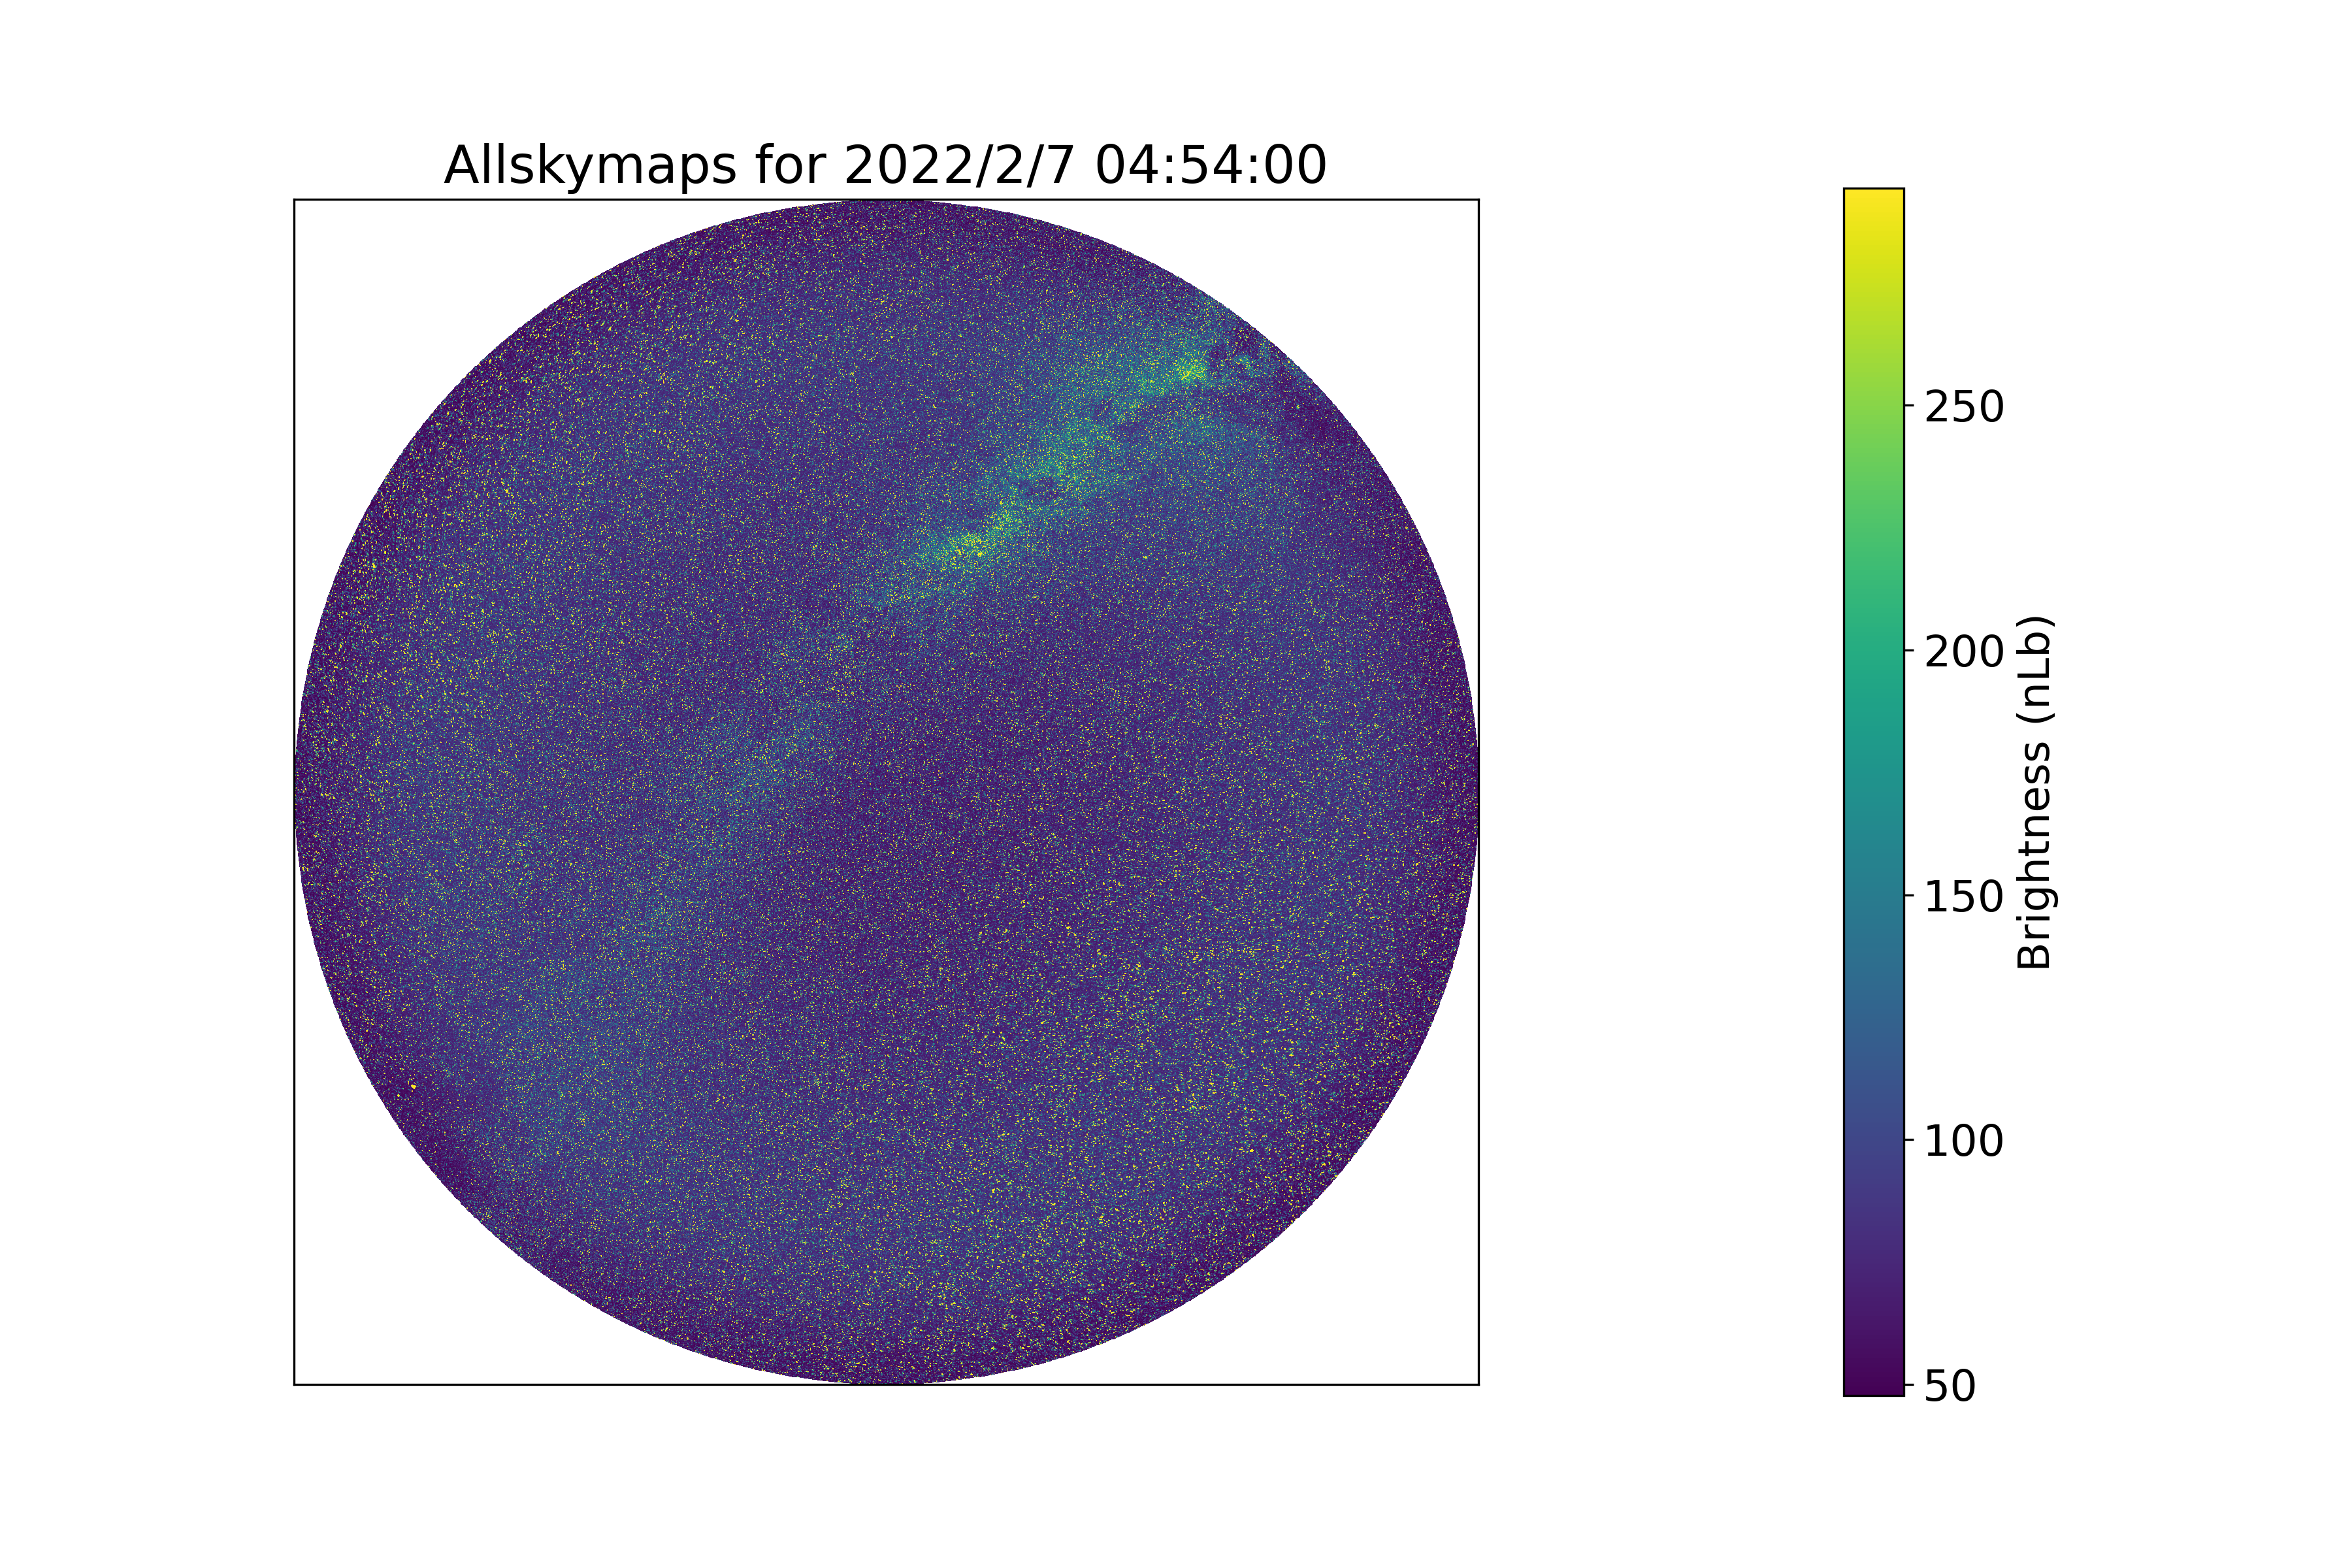
\includegraphics[width=1.0\columnwidth]{./figures/allskyetacardarkgauss3.png}
\caption{An map of the entire sky at the time of the Eta Carinae observations under astronomical dark time, generated using the \textit{hess\_basic} model in \textit{nsb} and our selected parameters. The galactic plane is clearly visible.}
\label{fig:allskyetacardarkgauss3}
\end{centering}
\end{figure}
As a reasonable worst-case scenario, we consider four observing scenarios of the colliding wind binary Eta Carinae. Eta Carinae has recently been the subject of a major paper by H.E.S.S. \cite{hessetacar}, and  is considered to be a particularly difficult $\gamma$-ray source to observe with IACTs given the high stellar density in the region and the high number of UV photons produced (which causes false triggers, though this is not taken into account by \textit{nsb}). Firstly we consider a `dark' field, at the same altitude as Eta Carinae but differing azimuth, for comparison. This appears to be a reasonable choice of dark field more generally, as there is only a single star with a V-band magnitude brighter than 3 (Zeta Centauri, $m_V=2.55$), though through a search of NASA's HEASARC catalogue there are 8 4FGL \textit{Fermi} LAT point sources in the dark field, which may have spectra that extend into the SST energy range (although this is unlikely as this is a high-galactic-latitude field meaning the 4FGL sources are likely blazars at high redshift). Secondly we consider observing Eta Carinae during astronomical dark time (at the same observing time as the dark field). Thirdly, we observe the Eta Carinae region with half moonlight present. This half moonlit scenario is designed to partially replicate the conditions for CTA requirement B-SST-1680, in this scenario the moon is above the horizon and has 0.53 Fractional Lunar Illumination (FLI). Finally we observe the region under full moonlight. The full moon scenario represents the worst possible observing conditions for Eta Carinae (and by extension the worst observing conditions possible), with the moon both at 1.0 FLI and well above the horizon. The significant all-sky illumination caused by this full moon, which completely dominates over the background stars, can be seen in Figure \ref{fig:allskyetacarextreme} (for comparison with the dark time all-sky plot in Figure \ref{fig:allskyetacardarkgauss3}).

In addition to pixel-wise analysis, we can also bin mean NSB values for these observations per superpixel and TM. This is important for understanding the triggering process, which relies on charge values per superpixel rather than per pixel, and for thermal control of the TM electronics (as each TM is thermally bonded to a chiller plate we need one temperature measurement per TM). These results can be seen in Figures \ref{fig:etacarpixel}, \ref{fig:etacarsuperpixel} and \ref{fig:etacarTM}. Because the camera trigger rate is reliant upon two adjacent superpixels exceeding a configurable threshold (as discussed in Chapter \ref{ch:1-intro}), the camera readout rates will be significantly lower than the NSB photon rates presented here for individual pixels. Here is a rough calculation that demonstrates this effect \cite{richpc}:

\begin{itemize}
    \item Let us assume the nominal NSB photon rate hitting an individual pixel is $40\,\mathrm{MHz}$ (the currently assumed SSTCAM rate \cite{richpc}).
    \item There are approximately 10,000 SiPM $\mu\textrm{cells}$ per pixel \cite{jasonthesis}, which means that the mean NSB photon rate per $\mu\textrm{cell}$ is $\sim4\,\mathrm{kHz}$.
    \item If SSTCAM is equipped with a digital trigger that requires approximately 10 $\mu\textrm{cells}$ to fire within the FWHM of our SiPM pulse length ($10.5\,\mathrm{ns}$), then the accidental trigger rate $A_{10}$ for 10 of our $\mu\textrm{cells}$ out of a total of $10,000\,\mu\textrm{cells}\times4$ (a single superpixel) is given by \cite{bradbury}
    \begin{equation}
        A_{10}=\frac{(4 \times 10,000)!}{10!(4 \times 10,000 - 10)!}(4\,\mathrm{kHz})^{10}(10.5\,\mathrm{ns})^{10-1} \approx 5\,\mathrm{kHz\ per\ superpixel}.
    \end{equation}
    \item Then as the backplane co-incidence trigger requires 2 neighbouring superpixels to trigger within $8\,\mathrm{ns}$ of each other, and there are 1910 combinations of our $2048/4=512$ superpixels that form neighbours, then the camera trigger rate $C_T$ is
    \begin{equation}
        C_T = 1910 \times (5\,\mathrm{kHz})^2 \times 8\,\mathrm{ns} \approx 380\,\mathrm{Hz}.
    \end{equation}
\end{itemize}
It should be noticed that this rough calculation is very sensitive to the superpixel trigger threshold and the selected TARGET ASIC co-incidence window. 

The results from our investigation are encouraging. For the dark field we compute a photon rate of $\mathrm{43\,MHz}$, a calculation performed by K. Bernlohr using \textit{sim\_telarray} by scaling the Benn and Ellison spectrum \cite{BandE} computes $\mathrm{41.9\,MHz}$. Assuming Poisson error these results are in agreement. Even for the worst case scenario the average photon rate is within SSTCAM observing requirements, though the combination of moonlight and a bright stars means pixels greater with an NSB rate of more than a few GHz will need to be disabled (or have their HV ramped down) and removed from Cherenkov analysis in order to manage SiPM heating. In the case of brighter stars illuminating a pixel at around a GHz it is likely such pixels will only be removed from the trigger analysis.
\begin{table}[t!]
    \centering
    \resizebox{\textwidth}{!}{

    \begin{tabular}{c|c|c|c|c|c}
         \textbf{Observation}&\textbf{Observing Time}&\textbf{ALT ($^{\circ}$)}&\textbf{AZ ($^{\circ}$)} & \textbf{RA ($^{\circ}$)}&\textbf{DEC ($^{\circ}$)} \\ 
         \hline
         Dark 'Empty' Field & 2022-02-07T04:54:0 & 33.1 & 126.7 & 162.0 & -43.0\\
         Eta Carinae No Moonlight &2022-02-07T04:54:0 & 33.1 & 146.7 &161.3&-59.7\\
         Eta Carinae Half Moonlight &20-02-21T01:10:0 & 12.5 & 150.8 &161.3&-59.7\\
         Eta Carinae Full Moonlight &2022-05-16T07:00:00& 13.1&209.6&161.3&-59.7
         
    \end{tabular}
    }
    \caption{Observation parameters for the four Eta Carinae Runs.  The observing Altitude (ALT) and Azimuth (AZ) are presented, along with the simulated source Right Ascension (RA) and Declination (DEC). The moonlit Eta Carinae runs are at a low altitude that an IACT would not normally observe at, but since the \textit{nsb} model does not contain a full atmospheric model this is inconsequential. Times are in UTC.}
    \label{tab:etacar_params}
\end{table}

\begin{figure}[t!]
\begin{centering}
%L, B, R, T
\includegraphics[width=1\columnwidth]{./figures/allskyetacarextreme.png}
\caption{An all-sky plot for the full moonlight run, highlighting the presence and brightness of the moon for this observation. \textit{nsb} performs an angular cut around the region of the moon when performing the all-sky-map calculation (resulting in the hole in this map).}
\label{fig:allskyetacarextreme}
\end{centering}
\end{figure}

%% Figure example 
\begin{figure}[t!]
%L, B, R, T
\begin{minipage}{\linewidth}\centering
\subcaptionbox{Dark empty field.}{\includegraphics[width=0.48\linewidth]{./figures/etacardarkgauss3_Hz_pixel.png}}
\subcaptionbox{No moonlight Eta Carinae.}{\includegraphics[width=0.48\linewidth]{./figures/etacarbrightgauss3_Hz_pixel.png}}
\subcaptionbox{Half moonlight Eta Carinae.}{\includegraphics[width=0.48\linewidth]{./figures/etacarmoonpoint53gauss3_Hz_pixel.png}}
\subcaptionbox{Full moonlight Eta Carinae.}{\includegraphics[width=0.48\columnwidth]{./figures/etacarnightmarev2_Hz_pixel.png}}
\caption{Per pixel NSB values for Eta Carinae under the four observing scenarios described.}
\label{fig:etacarpixel}

\end{minipage}
\end{figure} 

\begin{figure}[t!]
%L, B, R, T
\begin{minipage}{\linewidth}\centering
\subcaptionbox{Dark empty field.}{\includegraphics[width=0.48\linewidth]{./figures/Hz_Superpixel_dark.png}}
\subcaptionbox{No moonlight Eta Carinae.}{\includegraphics[width=0.48\linewidth]{./figures/Hz_Superpixel_bright.png}}
\subcaptionbox{Half moonlight Eta Carinae.}{\includegraphics[width=0.48\linewidth]{./figures/Hz_Superpixel_moonpoint53.png}}
\subcaptionbox{Full moonlight Eta Carinae.}{\includegraphics[width=0.48\columnwidth]{./figures/Hz_Superpixel_nightmare.png}}
\caption{Mean NSB values per superpixel for Eta Carinae under the four observing scenarios described.}
\label{fig:etacarsuperpixel}
\end{minipage}
\end{figure} 

\begin{figure}[t!]
%L, B, R, T
\begin{minipage}{\linewidth}\centering
\subcaptionbox{Dark empty field.}{\includegraphics[width=0.48\linewidth]{./figures/etacardarkgauss3_Hz_TM.png}}
\subcaptionbox{No moonlight Eta Carinae.}{\includegraphics[width=0.48\linewidth]{./figures/etacarbrightgauss3_Hz_TM.png}}
\subcaptionbox{Half moonlight Eta Carinae.}{\includegraphics[width=0.48\linewidth]{./figures/etacarmoonpoint53gauss3_Hz_TM.png}}
\subcaptionbox{Full moonlight Eta Carinae.}{\includegraphics[width=0.48\columnwidth]{./figures/etacarnightmarev2_Hz_TM.png}}
\caption{Mean NSB values per TM for Eta Carinae under the four observing scenarios described.}
\label{fig:etacarTM}
\end{minipage}
\end{figure} 


\subsection{Changes Between Adjacent Units for Eta Carinae}
\label{sec:etacarajacent}

We also re-analysed the data for the purposes of determining the maximum change between horizontally and vertically adjacent pixels, superpixels and TMs. This is necessary to predict the influence of stars on the camera trigger (for individual pixels), on bright NSB regions on the superpixel trigger logic, and for understanding the thermal load on the cooling plate bonded to each TM. This analysis was performed by devising a function that, for every pixel in a 2D array, obtains the maximum change in mean NSB rate between itself and its adjacent neighbours (if they exist), then assigns that value to the pixel. This calculation neglects changes in the PSF across the focal plane in the camera. The results from this investigation are shown in Figures \ref{fig:diffetacarpixel}, \ref{fig:diffetacarsuperpixel} and \ref{fig:diffetacarTM}.



\begin{figure}[t!]
%L, B, R, T
\begin{minipage}{\linewidth}\centering
\subcaptionbox{Dark empty field.}{\includegraphics[width=0.48\linewidth]{./figures/Hz_pixel_diff_dark.png}}
\subcaptionbox{No moonlight Eta Carinae.}{\includegraphics[width=0.48\linewidth]{./figures/Hz_pixel_diff_bright.png}}
\subcaptionbox{Half moonlight Eta Carinae.}{\includegraphics[width=0.48\linewidth]{./figures/Hz_pixel_diff_moonpoint53.png}}
\subcaptionbox{Full moonlight Eta Carinae.}{\includegraphics[width=0.48\columnwidth]{./figures/Hz_pixel_diff_nightmare.png}}
\caption{Maximum differences between adjacent pixels in NSB values for Eta Carinae under the four observing scenarios described.}
\label{fig:diffetacarpixel}

\end{minipage}
\end{figure} 

\begin{figure}[t!]
%L, B, R, T
\begin{minipage}{\linewidth}\centering
\subcaptionbox{Dark empty field.}{\includegraphics[width=0.48\linewidth]{./figures/Hz_Superpixel_diff_dark.png}}
\subcaptionbox{No moonlight Eta Carinae.}{\includegraphics[width=0.48\linewidth]{./figures/Hz_Superpixel_diff_bright.png}}
\subcaptionbox{Half moonlight Eta Carinae.}{\includegraphics[width=0.48\linewidth]{./figures/Hz_Superpixel_diff_moonpoint53.png}}
\subcaptionbox{Full moonlight Eta Carinae.}{\includegraphics[width=0.48\columnwidth]{./figures/Hz_Superpixel_diff_nightmare.png}}
\caption{Difference in mean NSB values between adjacent superpixels for Eta Carinae under the four observing scenarios described.}
\label{fig:diffetacarsuperpixel}

\end{minipage}
\end{figure} 

\begin{figure}[t!]
%L, B, R, T
\begin{minipage}{\linewidth}\centering
\subcaptionbox{Dark empty field.}{\includegraphics[width=0.48\linewidth]{./figures/Hz_TM_diff_dark.png}}
\subcaptionbox{No moonlight Eta Carinae.}{\includegraphics[width=0.48\linewidth]{./figures/Hz_TM_diff_bright.png}}
\subcaptionbox{Half moonlight Eta Carinae.}{\includegraphics[width=0.48\linewidth]{./figures/Hz_TM_diff_moonpoint53.png}}
\subcaptionbox{Full moonlight Eta Carinae.}{\includegraphics[width=0.48\columnwidth]{./figures/Hz_TM_diff_nightmare.png}}
\caption{Difference in mean NSB values between adjacent TMs for Eta Carinae under the four observing scenarios described.}
\label{fig:diffetacarTM}

\end{minipage}
\end{figure}

In the case of individual pixels, it appears the pixels adjacent to those with high NSB from stars are largely isolated from other potential sources of NSB, however once these results are binned and averaged by superpixel and TM that one starts to frequently observe the effect of multiple stars overlapping. The increased changes near the camera's uninstrumented corners are an analysis artefact stemming from the lack of pixel, TM and superpixels in these regions. However, it appears clear that pixels, superpixels and TMs need to be robust to a single pixel being at illuminated at a rate of $\mathrm{1\,GHz}$ whilst its neighbours are illuminated at a few hundred MHz.

\subsection{Change in Eta Carinae NSB Over Time}
To determine the maximum possible change in NSB through the camera over a run, we ran \textit{nsb} to simulate an observation of the instant exactly a half hour before each of the observations in Table \ref{tab:etacar_params} (tracking the source). This choice was based on the fact that the source sets after the full moonlight run, and also removes potential issues related to normalisation of pixel intensities in nLb over time that we discuss in the next subsection. Whilst these results in Figures \ref{fig:30minsetacarpixel}, \ref{fig:30minsetacarsuperpixel} and \ref{fig:30minsetacarTM} show that the brightness of an individual pixel can change on the order of a GHz per 30 minutes, changes in the mean illumination of the camera are much slower, being of the order of $\mathrm{2\,MHz/hour}$. This is with the exception of the fully moonlit scenario, where the mean change over half an hour is dominated by a bright star.

\begin{figure}[t!]
%L, B, R, T
\begin{minipage}{\linewidth}\centering
\subcaptionbox{Dark empty field.}{\includegraphics[width=0.48\linewidth]{./figures/diff_Hz_pixel_dark.png}}
\subcaptionbox{No moonlight Eta Carinae.}{\includegraphics[width=0.48\linewidth]{./figures/diff_Hz_pixel_bright.png}}
\subcaptionbox{Half moonlight Eta Carinae.}{\includegraphics[width=0.48\linewidth]{./figures/diff_Hz_pixel_moonpoint53.png}}
\subcaptionbox{Full moonlight Eta Carinae.}{\includegraphics[width=0.48\columnwidth]{./figures/diff_Hz_pixel_nightmare.png}}
\caption{Changes in Eta Carinae NSB values per pixel over 30 minutes.}
\label{fig:30minsetacarpixel}

\end{minipage}
\end{figure} 

\begin{figure}[t!]
%L, B, R, T
\begin{minipage}{\linewidth}\centering
\subcaptionbox{Dark empty field.}{\includegraphics[width=0.48\linewidth]{./figures/diff_Hz_Superpixel_dark.png}}
\subcaptionbox{No moonlight Eta Carinae.}{\includegraphics[width=0.48\linewidth]{./figures/diff_Hz_Superpixel_bright.png}}
\subcaptionbox{Half moonlight Eta Carinae.}{\includegraphics[width=0.48\linewidth]{./figures/diff_Hz_Superpixel_moonpoint53.png}}
\subcaptionbox{Full moonlight Eta Carinae.}{\includegraphics[width=0.48\columnwidth]{./figures/diff_Hz_Superpixel_nightmare.png}}
\caption{Changes in Eta Carinae NSB values per superpixel over 30 minutes.}
\label{fig:30minsetacarsuperpixel}

\end{minipage}
\end{figure} 

\begin{figure}[t!]
%L, B, R, T
\begin{minipage}{\linewidth}\centering
\subcaptionbox{Dark empty field.}{\includegraphics[width=0.48\linewidth]{./figures/diff_Hz_TM_dark.png}}
\subcaptionbox{No moonlight Eta Carinae.}{\includegraphics[width=0.48\linewidth]{./figures/diff_Hz_TM_bright.png}}
\subcaptionbox{Half moonlight Eta Carinae.}{\includegraphics[width=0.48\linewidth]{./figures/diff_Hz_TM_moonpoint53.png}}
\subcaptionbox{Full moonlight Eta Carinae.}{\includegraphics[width=0.48\columnwidth]{./figures/diff_Hz_TM_nightmare.png}}
\caption{Changes in Eta Carinae NSB values per TM over 30 minutes.}
\label{fig:30minsetacarTM}
\end{minipage}
\end{figure} 
A procedure to deal with the moon entering the FoV (potentially by accident) has not yet been established for SSTCAM (one option is to pre-emptively drop the gain for the entire camera). However, attempting to run NSB for an observation whereby the moon is directly in the field crashes \textit{nsb}. As such, the change in the full moonlit Eta Carinae field represents the greatest shift in average NSB rate that can be simulated ($\mathrm{30\,MHz/Minute/pixel}$) with \textit{nsb}.

\subsection{Eta Carinae NSB Per Pixel}
\label{sec:etacartimespan}
\begin{figure}[t!]
\begin{centering}
%L, B, R, T
\resizebox{\columnwidth}{!}{\includegraphics[width=\columnwidth]{./figures/etacartimespan.png}}
\caption{Pixel brightness in Hz for Eta Carinae over a year, normalised to a mean observing rate of 76Hz.}
\label{fig:etacar_timespan}
\end{centering}
\end{figure}

\textit{nsb} has a tool to determine the limit of brightness in a single pixel over a year. However, said tool only provides results in nLb at a particular infinitesimal point, which is something of a meaningless quantity. As such, for running this tool for SSTCAM with NSB, we assume our non-moonlight Eta Carinae NSB run from Section \ref{sec:etacarvary} represents a typical observation, and scale the mean of the year long timespan plot to the mean pixel value for that run. In the case of the maximum NSB variation over a single night, we instead normalise the maximum of the NSB rate to the maximum of the year long plot (to which the single night's observation corresponds).

Figure \ref{fig:etacar_timespan} clearly shows that whilst there is modulation in the apparent brightness of the region given lunar phase and separation, there is also a very strong dependence on moon altitude, with the brightest times being when the moon is both high on the sky, near $\mathrm{1.0\,FLI}$, and close to the source. Throughout these results and those in Subsection \ref{sec:etacarvary} it appears as though lunar illumination, separation and altitude will be the dominant cause of both high NSB and rapid changes in it.

There is some inconsistency between this result and the result for the entire camera on the same night with a 30 minute difference, which shows an overall drop in NSB over the same time window, although both show extreme variation. This could be the result of a minor bug in \textit{nsb}, or it could be a results of the infinitesimally small region of the sky corresponding to Eta Carinae brightening whilst the larger FoV is darkening. However, this suggests that even on the most extreme sources changes in NSB rate per pixel should be within the capacity of the LED flasher system to correct. 

\begin{figure}[t!]
\begin{centering}
%L, B, R, T
\resizebox{\columnwidth}{!}{\includegraphics[trim=0cm 0cm 0cm 0cm,clip=true,width=\columnwidth]{./figures/timespan_Hz_etacarmaxnorm.png}}
\caption{Pixel brightness in Hz for Eta Carinae for the brightest observing night in 2022, normalised to a $\mathrm{264.8\,}$Hz max observation rate (as determined from Figure \ref{fig:etacar_timespan}).}
\label{fig:etacar_timespan_extreme}
\end{centering}
\end{figure}
\newpage
\subsection{Observing Time Gains}
Within \textit{nsb}, there is similarly a function to provide plots of the observation time gained as a function of NSB threshold, but this again is in nLb at an infinitesimal point. As such, we treat our Eta Carinae dark frame as nominal, and create a timespan plot for that night (shown in Figure \ref{fig:timespan_dark} and observing location. The total possible observing time is obtained by summing all the elements in the brightness array where the brightness is less than a given threshold , and then multiplying this by the time resolution (as the time resolution for this brightness array is a pre-set parameter).
\begin{figure}[t!]
\begin{centering}
%L, B, R, T
\resizebox{\columnwidth}{!}{\includegraphics[trim=0cm 0cm 0cm 0cm,clip=true,width=\columnwidth]{./figures/timespan_dark.png}}
\caption{NSB timespan plot for the dark field used to calibrate the observing time gain calculation. The CTA SST operation requirement (up to 18x nominal NSB) is also shown.}
\label{fig:timespan_dark}
\end{centering}
\end{figure}

We then divide the observation time gain values by a the nominal NSB value obtained from this measurement ($\mathrm{50\,nLb}$), and perform an observing time gain calculation for the Vela Pulsar (Figure \ref{fig:obstimegainvelapulsar}) and the blazar Markarian 421 (Figure \ref{fig:obstimegainmrk421}, in order to consider differences from galactic versus extragalactic sources) from the Paranal site, considering a year at the Paranal site starting at 2022-01-27. The associated CTA requirement is also shown in these figures.

\begin{figure}[h!]
\begin{centering}
%L, B, R, T
\includegraphics[width=\columnwidth]{./figures/obstime_VelaPulsar_nom.png}
\caption{Observing time gain for the Vela Pulsar as a function of nominal NSB.}
\label{fig:obstimegainvelapulsar}
\end{centering}
\end{figure}

\begin{figure}[h!]
\begin{centering}
%L, B, R, T
\includegraphics[width=\columnwidth]{./figures/obstime_mrk421_nom.png}
\caption{Observing time gain for Markarian 421 as a function of nominal NSB.}
\label{fig:obstimegainmrk421}
\end{centering}
\end{figure}

Whilst the potential observation time gains for the Vela Pulsar are significant, the potential benefits of operating at a higher NSB rate are more muted for Markarian 421. This is partly due to the location of the Paranal site, and as such Markarian 421 is typically lower on the sky, but it is also likely that the fact that Markarian 421 is away from the galactic plane (with fewer stars in the field) contributes to this. This therefore bodes well for potential SSTCAM galactic transient science, such as observations of the recurrent nova RS Ophiuchi (recently detected by H.E.S.S. in ATEL 14857). 

\subsection{Exact Matching of Half-Moonlight Requirement}
Whilst a reasonable approximation given the complexity of observing a particular source, the half-moonlight Eta Carinae runs are not an exact match to the CTA SST Requirement B-SST-1680, which states
\begin{quote}
    \textit{SSTs must be capable of $\gamma$-ray observations with uniform night sky background illumination levels up to at least $\mathit{4.3}\ photons\ ns^{-1} sr^{-1} cm^{-2}$ in the wavelength range $\mathit{300-650}\,nm$ with the Moonlight Reference Spectrum.}
\end{quote}
Additionally, this requirement mandates that the moon must be at $\mathrm{0.5\,FLI}$ and is at an altitude of 45 degrees and the telescope is pointed at the zenith. To compare to our half-moonlit Eta Carinae run, we ran \textit{nsb} runs with exactly these parameters for UTC time 2022-03-24T07:32:00.000, the results from this investigation are shown in Figure \ref{fig:hm}.

\begin{figure}[t!]
%L, B, R, T
\begin{minipage}{\linewidth}\centering
\subcaptionbox{NSB per pixel.}{\includegraphics[width=0.48\linewidth]{./figures/hm_pixel.png}}
\subcaptionbox{NSB per superpixel.}{\includegraphics[width=0.48\linewidth]{./figures/hm_Superpixel.png}}
\subcaptionbox{NSB per TM.}{\includegraphics[width=0.48\linewidth]{./figures/hm_TM.png}}

\caption{Results for half-moonlit zenith observations.}
\label{fig:hm}

\end{minipage}
\end{figure}
The results for these half-moonlight observations demonstrate that if SSTCAM performance requirements up to a $\mathrm{160\,MHz}$ NSB rate can be met, the overall camera will function well under most realistic observing scenarios. The question becomes if individual pixels will be able to handle such NSB rates without an overwhelming gain$\times$PDE$\times$Optical Cross-Talk (OCT) drop. Whilst in general we want OCT (a phenomenon caused by infrared secondary photons generated during the electron avalanche escaping their SiPM channels) to be as low as possible, as all three of these quantities are proportional to $\Delta V$; if we reduce the overvoltage to minimise the OCT we will degrade the camera's performance.

These half-moonlit results are slightly more pessimistic than the half-moonlit Eta-Carinae runs, due to the difficulty of observing Eta Carinae at the requirement altitude from the southern site, but they are still within a factor of around 2 of the same values. They are also largely consistent with values generated using \textit{sim\_telarray}; for the simulation production Prod3b \textit{sim\_telarray} predicts between 160 and 200MHz (depending on SiPM selection). This \textit{sim\_telarray} prediction is based on scaling the Benn and Ellison spectrum under the same conditions. In contrast, the existing half-moonlight investigation for the SST-1M project \cite{1mcalib} estimated a value of $\mathrm{670\,MHz}$ for the same conditions. Other than human error a possible source of this discrepancy is the physical size of the photomultiplier pixels, which for SSTCAM is $\mathrm{6/7\,mm}$ ($0.19^{\circ}$ on sky) as opposed to around $\mathrm{2.32\,cm}$ ($0.24^{\circ}$ on sky) for Digicam (the SST-1M prototype camera). Other differences between the photomultipliers used (such as PDE) might also affect the Digicam results. 

\subsection{Required Flasher Timespans}

The complexity of operating a fast-signal chain for Cherenkov astronomy simultaneously with a slow-signal chain for pointing validation is a problem unique to SSTCAM, and implementing this requires that the effect of bright stars upon the telescope calibration is well understood. In the next three subsections, we will attempt to better understand the effects of such stars upon SSTCAM calibration.

The angular field rotation of a star $R$ can be described as a function of Latitude (Lat), Altitude (Alt) and Azimuth (Az) using the formula
\begin{equation}
    R(\mathrm{Lat,Alt,Az})=K\cos(\mathrm{Lat})\frac{\cos(\mathrm{Az})}{\cos(\mathrm{Alt)}}
    \label{eq:rot}
\end{equation}
where the constant $K$ is $\mathrm{15.04\,degrees/hour}$. Using this formula, it is possible to extract the number of required flasher calibration pulses to reach a mean flasher error level. If we assume a mean illumination level from the flasher of $50\,\mathrm{photoelectrons}$ (pe), and that the Excess Noise Factor (ENF), a property of the SiPMs used that describes the physical limit for the best possible SiPM charge resolution \cite{jasonthesis}, is 1.4 (the physically un-reachable ideal limit at which the charge resolution is limited by Poisson fluctuations would be 1). Then we need $40\,\mathrm{s}$ (i.e. $400\,\mathrm{pulses}$) to reach a 1\% error on the mean flasher level per pixel. This is the needed flasher calibration level for SSTCAM to be able to meet the intensity resolution requirements of CTA for high-amplitude signals, details of this intensity resolution requirement can be found in \cite{tomintensity}. The limits on stellar rotation rate occur at the point at which stars cause a gain change in a SiPM pixel that happens more rapidly than can be calibrated for by injecting flashes at a fixed rate.

Figure \ref{fig:rot40s} shows the areas on the sky where a 1\% flasher error can be achieved given this model of angular field rotation. The sky positions (assuming the Paranal site) of bright stars (brighter than 4 mag) from the \textit{Hipparcos} catalogue are calculated using the \textit{Skyfield} package and are also plotted.
\begin{figure}[t!]
\begin{centering}
%L, B, R, T
\includegraphics[width=0.7\columnwidth]{./figures/rot40s.png}
\caption{Field rotation with flasher calibration limit, assuming 40s flasher calibration intervals.}
\label{fig:rot40s}
\end{centering}
\end{figure}

This clearly causes a slight error in calibration along the North-South axis, but this is tolerable given the rate at which stars move across the sky. By doubling the error budget and reducing the between the flashing procedure one can achieve much greater calibrated sky coverage, as seen in Figure \ref{fig:rot10s}, with only a handful of bright stars falling outside the calibrated range. These results suggest that the current flasher calibration plan for SSTCAM of using the flasher to generate 100-200 photons with nanosecond precision \footnote{Further details of this (early) calibration plan can be found on the internal SSTCAM nextcloud pages at \url{https://pcloud.mpi-hd.mpg.de/index.php/apps/files/?dir=/SSTCamera/03_CameraCalls/CameraCallMaterial&openfile=305207}.} is likely to be acceptable.

\begin{figure}[t!]
\begin{centering}
%L, B, R, T
\includegraphics[width=0.7\columnwidth]{./figures/rot10s.png}
\caption{Field rotation with flasher calibration limit, assuming 10s flasher calibration intervals.}
\label{fig:rot10s}
\end{centering}
\end{figure}

\subsection{Star Tracking Investigations}

To understand the short-term effect of stars moving through the field, we ran \textit{nsb} fields at 3 minute intervals, pointing at the zenith under half-moonlit conditions, and observed both the absolute pixel NSB values and the overall change since the first field. Note that this is also a worst-case scenario observing the fastest possible changes in stellar position, since $R$ in Equation \ref{eq:rot} is largest for a given observing latitude at the zenith.

Despite the PSF not being particularly well modelled, it appears that bright stars move to adjacent pixels over a roughly 15 minute timespan, with light being partially `split' between multiple pixels and the associated ratio changing over order 3 minutes.
\begin{figure}[t!]
%L, B, R, T
\begin{minipage}{\linewidth}\centering
\subcaptionbox{Initial field.}{\includegraphics[width=0.48\linewidth]{./figures/Hz_pixel_3m.png}}
\subcaptionbox{Pixel values after 3 minutes.}{\includegraphics[width=0.48\linewidth]{./figures/Hz_pixel_6m.png}}
\subcaptionbox{Pixel values after 6 minutes.}{\includegraphics[width=0.48\linewidth]{./figures/Hz_pixel_9m.png}}
\subcaptionbox{Pixel values after 9 minutes.}{\includegraphics[width=0.48\columnwidth]{./figures/Hz_pixel_12m.png}}
\subcaptionbox{Pixel values after 12 minutes.}{\includegraphics[width=0.48\columnwidth]{./figures/Hz_pixel_15m.png}}

\caption{Pixel NSB Values in Hz, pointing at the zenith under `half-moonlit' conditions with high resolution timing, note in particular the changes to the three brightest pixels in the images.}

\end{minipage}
\label{fig:zenithpixel}
\end{figure} 

\begin{figure}[t!]
%L, B, R, T
\begin{minipage}{\linewidth}\centering
\subcaptionbox{Total change in pixel values after 3 minutes.}{\includegraphics[width=0.48\linewidth]{./figures/diff_Hz_pixel_3m.png}}
\subcaptionbox{Total change in pixel values after 6 minutes.}{\includegraphics[width=0.48\linewidth]{./figures/diff_Hz_pixel_6m.png}}
\subcaptionbox{Total change in pixel values after 9 minutes.}{\includegraphics[width=0.48\linewidth]{./figures/diff_Hz_pixel_9m.png}}
\subcaptionbox{Total change in pixel values after 12 minutes.}{\includegraphics[width=0.48\columnwidth]{./figures/diff_Hz_pixel_12m.png}}

\caption{Overall change in pixel NSB values in Hz for the high time resolution star tracking investigation.}

\end{minipage}
\label{fig:zenithpixelchange}
\end{figure} 

\subsection{Results for Observations of a Magnitude 0 star}
For upcoming comparisons with other ray-tracing simulation methods, we investigated the brightness of Rigel (m=0.12) under astronomical dark time (UTC time 2021-12-08T04:48:00.000). This shows the light from a magnitude 0 star corresponds to an NSB rate of around $\mathrm{900\,MHz}$ in a single pixel (lower than previously expected). The movement of the star through multiple pixels in the camera plane could affect this value as seen in the previous subsection.
\begin{figure}[t!]
\begin{centering}
%L, B, R, T
\includegraphics[width=0.7\columnwidth]{./figures/Hz_pixel_Rigel.png}
\caption{Rigel observed with \textit{nsb} under astronomical dark time conditions.}
\label{fig:rigel}
\end{centering}
\end{figure}
\section{Conclusions}

In this chapter, we have examined the potential effects of NSB for SSTCAM. We have presented detailed simulations of the background to Eta Carinae under four observing scenarios, calculated the effect on individual pixels observing the same field over time, calculated the potential observing time to be gained for two sources by operating at a high NSB level, verified the half moonlight CTA requirement, investigated on short timescales the movement of stars through the camera and considered the ability of the LED flasher system to compensate for NSB from stars.

Whilst the \textit{nsb} package has proven capable of generating useful results for SSTCAM, it currently does not meet CTA software requirements for test coverage or code quality (and development by H.E.S.S. on the package has stalled). There would be significant advantages to recreating its functionality in the future with a \textit{ctapipe}-affiliated project (following modern code development principles) for all CTA instruments. Notably \textit{nsb}'s speed could likely be improved by using Just-In-Time compilation and a storage medium for healpix data that was quicker to access and parse than a text file (as is currently the case).

It should be noted that the results presented here are a significantly simplified analysis. In particular, we do not consider the effects of OCT, focal plane curvature or non-uniformity of the PSF across the camera plane. Similarly, there is a potential for `ghost' stars to appear in the field of view as a result of reflections of starlight from the SiPMs or window. We also neglect any wavelength dependence of PDE or telescope transmission. That said, our models are significantly more realistic than those available natively in \textit{sim\_telarray}, are broadly as expected, and appear to be largely consistent with values obtained from dedicated full Monte Carlo simulations.


%%%%%%%%%%%%%%%%%%%%%%%%%%%%%%
%%%%% Appendices
%%%%%%%%%%%%%%%%%%%%%%%%%%%%%%

